%SourceDoc ws-skript.tex
%
% c04-verteilung.tex
%
% (c) 2006 Prof. Dr. Andreas M�ller
% $Id: c04b-verteilung.tex,v 1.9 2007/11/16 17:40:11 afm Exp $
%
\section{Diskrete Wahrscheinlichkeitsverteilungen}
Neben den vielen praktisch wichtigen stetigen Verteilungen
gibt es auch ein mindestens genauso lange Liste bedeutender
diskreter Verteilungen.
\subsection{Gleichverteilung\label{section-gleichverteilung-diskret}}
\index{Gleichverteilung!Erwartungswert}
\index{Gleichverteilung!Varianz}
\index{Gleichverteilung!Verteilungsfunktion}
\begin{table}
\renewcommand{\arraystretch}{1.5}
\begin{center}
\begin{tabular}{|l|l|}
\hline
Name&diskrete Gleichverteilung\\
\hline
Wahrscheinlichkeit&
\begin{minipage}{3.7in}
\vskip3pt
$\displaystyle P(k)=\frac1n$
\end{minipage}
\\
Verteilungsfunktion&
\begin{minipage}{3.7in}
$\displaystyle
\begin{cases}
0&\qquad x \le 1\\
{\displaystyle \frac{\left\lfloor x\right\rfloor}n}&\qquad 1\le x\le n
\\
1&\qquad x \ge n
\end{cases}
$
\end{minipage}
\\[30pt]
Erwartungswert&$\displaystyle \frac{n+1}2$\\[8pt]
Varianz&$\displaystyle \frac{n^2-1}{12}$\\[8pt]
Median&$\displaystyle \frac{n+1}2$\\[8pt]
\hline
Anwendungen&\begin{minipage}{3.7in}%
\vskip3pt
\strut
$\bullet$ Laplace-Ereignisse aller Art\\
$\bullet$ W"urfel\\
$\bullet$ Roulette
\strut
\end{minipage}\\[17pt]
\hline
\end{tabular}
\end{center}
\caption{Datenblatt der diskreten Gleichverteilung\label{datenblatt:diskretegleichverteilung}}
\end{table}

\begin{figure}
\centering
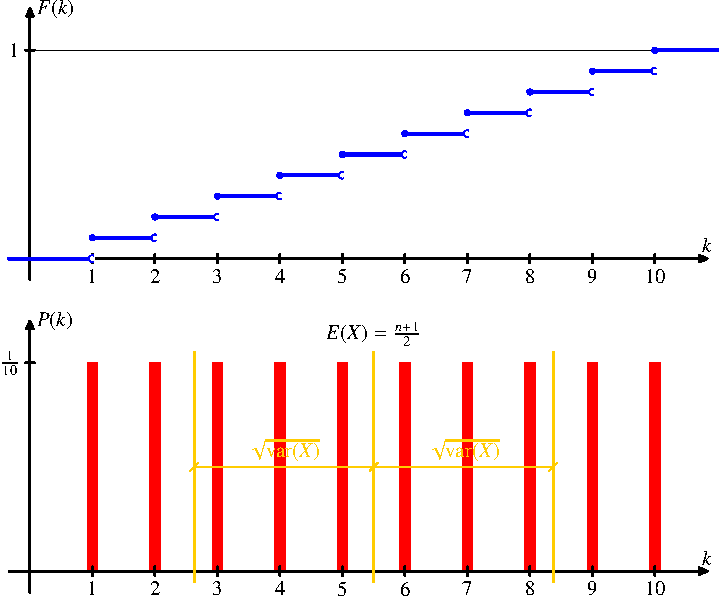
\includegraphics{images/gl-2.pdf}
\caption{Wahrscheinlichkeit und Verteilungsfunktion der diskreten Gleichverteilung
f"ur $n=10$
\label{graph-diskrete-gleichverteilung}}
\end{figure}

Bereits in Abschnitt \ref{section-laplace-ereignisse}
wurden endliche Wahrscheinlichkeitsr"aume
untersucht, bei denen alle Elementarereignisse mit gleicher Wahrscheinlichkeit
eingetreten sind. Im Kontext einer Zufallsvariable bedeutet
Gleichverteilung, dass jeder m"ogliche Wert mit gleicher Wahrscheinlichkeit
vorkommt. Im einfachsten Fall sind die Werte nat"urliche Zahlen
$\{1,\dots,n\}$, die Wahrscheinlichkeit f"ur den Wert ist 
$p(k)=\frac1n$. Die Verteilungsfunktion dieser Verteilung ist
\[
F(x)=
\begin{cases}
0&\qquad x \le 1\\
{\displaystyle \frac{\left\lfloor x\right\rfloor}n}&\qquad 1\le x\le n\\
1&\qquad x \ge n
\end{cases}
\]
Entsprechend einfach sind Erwartungswert und Varianz zu berechnen:
\begin{eqnarray*}
E(X)&=&\sum_{k=1}^nkp(k)=\frac1n\sum_{k=1}^nk=\frac1n\cdot\frac{n(n+1)}{2}=\frac{n+1}2\\
E(X^2)&=&\sum_{k=1}^nk^2p(k)=\frac1n\sum_{k=1}^nk^2=\frac1n\cdot\frac{n(1+3n+2n^2)}{6}=\frac{2n^2+3n+1}{6}\\
\operatorname{var}(X)&=&E(X^2)-E(X)^2=\frac{2n^2+3n+1}{6}-\frac{(n+1)^2}4\\
&=&\frac{4n^2+6n+2-3n^2-6n-3}{12}=\frac{n^2-1}{12}
\end{eqnarray*}
Die Wahrscheinlichkeit und die Verteilungsfunktion ist in
Abbildung~\ref{graph-diskrete-gleichverteilung} dargestellt.

\subsection{Binomialverteilung\label{section-binomialverteilung}}
\index{Bernoulli-Experiment}
\begin{table}
\renewcommand{\arraystretch}{1.5}
\begin{center}
\begin{tabular}{|l|l|}
\hline
Name&Binomialverteilung\\
\hline
Wahrscheinlichkeit&
\begin{minipage}{3.7in}
\vskip3pt
$\displaystyle P(k)=\binom{n}{k}p^k(1-p)^{n-k}$
\end{minipage}
\\[10pt]
Verteilungsfunktion&
$\displaystyle F(k)=\sum_{i=0}^k\binom{n}{i}p^i(1-p)^{n-i}$
\\[10pt]
Erwartungswert&$\displaystyle np$\\
Varianz&$\displaystyle np(1-p)$\\
\hline
Anwendungen&\begin{minipage}{3.7in}%
\strut
$\bullet$ Anzahl Eintreten eines Bernoulli-Experimentes
\strut
\end{minipage}\\
\hline
\end{tabular}
\end{center}
\caption{Datenblatt der Binomialverteilung\label{datenblatt:binomialverteilung}}
\end{table}
\begin{figure}
\centering
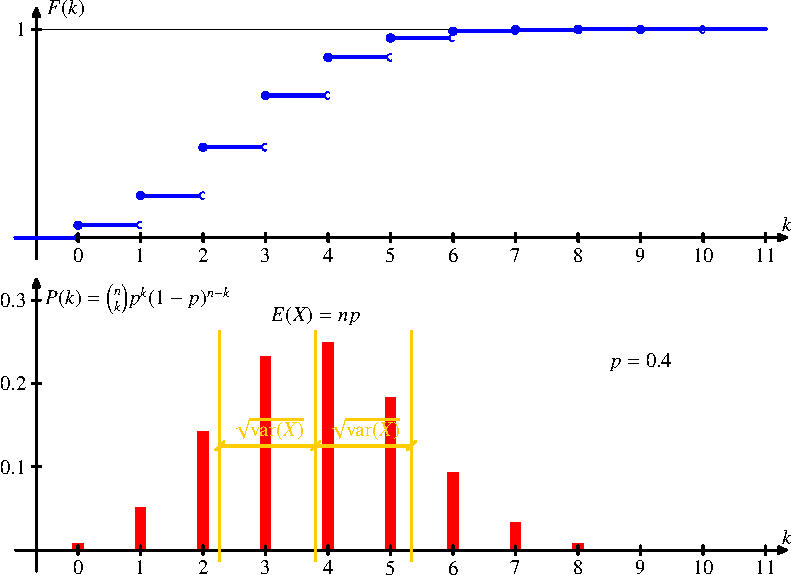
\includegraphics{images/gl-3.pdf}
\caption{Wahrscheinlichkeitsverteilung und Verteilungsfunktion einer
Binomialverteilung mit $p=0.4$ und $n=10$.
\label{binomialgraph}}
\end{figure}

Der Wurf einer M"unze ist der Spezialfall eines Versuches mit
zwei m"oglichen Ausg"angen $\{0,1\}$, bei dem die beiden Ausg"ange als
gleich wahrscheinlich angesehen werden. Es sind durchaus auch
Anwendungsf"alle denkbar, in denen die beiden Ausg"ange unterschiedliche
Wahrscheinlichkeit haben, zum Beispiel $p$ f"ur den Ausgang $1$ und $1-p$
f"ur $0$.
Ein solches Experiment nennt man ein Bernoulliexperiment.

Wir wiederholen jetzt dieses Experiment $n$ mal und betrachten die Ereignisse,
dass in genau $k$ der $n$ F"alle der Ausgang $1$ eingetreten ist,
und $0$ in allen anderen F"allen. Es gibt $\binom{n}{k}$ M"oglichkeiten,
die $k$ $1$-Experimente auszuw"ahlen, und die Kombination, dass genau
dieses Kombination $1$ und $0$ realisiert wird, ist $p^k(1-p)^{n-k}$.
Somit ist die Wahrscheinlichkeit, dass von $n$ Experimenten deren $k$
erfolgreich sind
\[
\binom{n}{k}p^k(1-p)^{n-k}.
\]
Dies ist die Binomialverteilung:
\index{Binomialverteilung}
\begin{definition}
Eine Zufallsvariable mit diskreten Werten $k\in\{0,\dots,n\}$
heisst binomialverteilt zum Parameter $p$, wenn die Wahrscheinlichkeit
des Wertes $k$ 
\[
\binom{n}{k}p^k(1-p)^{n-k}
\]
ist.
\end{definition}

Die Wahrscheinlichkeitsverteilung und die Verteilungsfunktion der
Binomialverteilung ist in Abbildung~\ref{binomialgraph} dargstellt.

\subsubsection{Erwartungswert und Varianz}
\index{Erwartungswert!der Binomialverteilung}
\index{Binomialverteilung!Erwartungswert}
Aus der bekannten Wahrscheinlichkeitsverteilung l"asst sich
Erwartungswert und Varianz berechnen:
\begin{satz}
Eine auf $\{0,\dots,n\}$ zum Parameter $p$ binomialverteilte Zufallsvariable
$X$ hat Erwartungswert
\[
E(X)=pn
\]
und Varianz
\[
\operatorname{var}(X)=np(1-p).
\]
Die maximale Varianz wird erreicht bei $p=\frac12$.
\end{satz}
\index{Varianz!der Binomialverteilung}
\index{Binomialverteilung!Varianz}

\begin{proof}[Beweis] Wir m"ussen die Summen
\begin{eqnarray*}
E(X)&=&\sum_{k=0}^nk\binom{n}{k}p^k(1-p)^{n-k}\\
E(X^2)&=&\sum_{k=0}^nk^2\binom{n}{k}p^k(1-p)^{n-k}
\end{eqnarray*}
berechnen k"onnen. Dazu betrachten wir die Hilfsfunktion
\[
f(x)=(x+y)^n=\sum_{k=0}^n\binom{n}{k}x^ky^{n-k},
\]
offensichtlich erhalten wir die Summe der Wahrscheinlichkeiten aller
binomailverteilten Werte, wenn
wir $x=p$ und $y=(1-p)$ einsetzen.
Die Ableitung nach $x$ gefolgt von Multiplikation mit $x$ liefert
\[
 x\frac{d}{dx}f(x)
=xn(x+y)^{n-1}\\
=\sum_{k=0}\binom{n}{k}kx^ky^{n-k}
\]
Nach Einsetzen von $x=p$ und $y=1-p$ entsteht rechts genau
der gesuchte Erwartungswert, links aber
\[
pn(p+1-p)^{n-1}=pn=\sum_{k=0}^n\binom{n}{k}kp^k(1-p)^{n-k}=E(X).
\]
Erneute Anwendung von $x\frac{d}{dx}$ liefert
\[
xn(x+y)^{n-1}+x^2 n(n-1)x^{n-2}=\sum_{k=0}^n\binom{n}{k}k^2x^ky^{n-k},
\]
und nach Einsetzen der Werte f"ur $x$ und $y$
\[
pn+p^2n(n-1)=\sum_{k=0}^n\binom{n}{k}k^2p^k(1-p)^{n-k}=E(X^2).
\]
Daraus bestimmen wir die Varianz
\[
\operatorname{var}(X)=E(X^2)-E(X)^2=pn+p^2n(n-1)-p^2n^2=p(1-p)n
\]
Die Funktion $p\mapsto np(1-p)$ ist eine quadratische Funktion mit den
Nullstellen $0$ und $1$. Quadratische Funktionen sind symmetrisch um
die Abszisse des Scheitelpunktes, der demzufolge in der Mitte zwischen
den Nullstellen bei $\frac12$ sein muss.
\end{proof}

\subsubsection{Der Grenzwert $n\to\infty$}
\index{Binomialverteilung!Normalapproximation}
Was geschieht, wenn die Zahl $n$ der Versuche beliebig vergr"ossert wird?
nat"urlich wird die Zahl der m"oglichen Werte der Zufallsvariable
gr"osser, der Erwartungswert $np$ und die Varianz $np(1-p)$ steigen.
Standardisiert man die Verteilung jedoch, indem man die Zufallsvariable
durch $Y=(X-np)/\sqrt{np(1-p)}$ ersetzt, dann wird die Zufallsvariable $Y$
Erwartungswert $0$ und Varianz $1$ haben. 

Durch die Skalierung r"ucken die m"oglichen Werte von $Y$ n"aher zusammen,
so dass man die Wahrscheinlichkeiten nicht direkt vergleichen kann.
Man kann aber die Verteilungsfunktionen $F_Y$ f"ur verschiedene Werte
von $n$ vergleichen. Aus dem zentralen Grenzwertsatz erh"alt man
jedoch die Aussage, dass die Verteilungsfunktion gegen die
Verteilungsfunktion der Standardnormalverteilung konvergieren wird.
Dieser Spezialfall des zentralen Grenzwertsatzes heisst auch der
Satz von de Moivre und Laplace.

Die Gr"osse $Y=(X-np)/\sqrt{np(1-p)}$ sollte also normalverteilt sein
mit Erwartungswert $0$ und Varianz $1$, aber nat"urlich nur, wenn $p$
tats"achlich die Wahrscheinlichkeit des einen Ausgangs des
Bernoulliexperimentes ist. Daraus l"asst sich jetzt ein Test daf"ur
konstruieren, ob $p$ die Wahrscheinlichkeit des einen Ausgangs eines
Bernoulliexperimentes ist. Ist $p$ n"amlich nicht die richtige
Wahrscheinlichkeit, wird f"ur grosse $Y$ mit grosser Wahrscheinlichkeit
stark von $0$ abweichen, es muss also nur ein Kriterium gefunden werden,
welches angibt, dass die Abweichung zu gross ist, um immer noch daran
zu glauben, dass das $p$ richtig war.

Ein rationales Kriterium l"asst sich mit der $\chi^2$-Verteilung konstruieren.
$Y^2$ ist $\chi^2$-verteilt mit einem Freiheitsgrad.
Die Wahrscheinlichkeit, dass $Y^2$ gr"osser ist als $M$ ist
\[
P(Y^2>M)=\int_M^\infty f_{\frac12,\frac12}(t)\,dt.
\]
Wenn wir also $M$ bestimmen, so dass diese Wahrscheinlichkeit 
zum Beispiel 5\% ist, dann glauben wir nicht mehr, dass $p$ tats"achlich
die Wahrscheinlichkeit des einen Ausgangs ist, sobald $Y^2>M$ wird,
und nur in 5\% aller F"alle werden wir dies zu unrecht tun.

\subsection{Hypergeometrische Verteilung\label{section-hypergeometrischeverteilung}}
\index{hypergeometrische Verteilung}
\index{hypergeometrische Verteilung!Erwartungswert}
\index{hypergeometrische Verteilung!Varianz}
\index{Varianz!hypergeometrische Verteilung}
\index{Erwartungswert!hypergeometrische Verteilung}
\begin{table}
\renewcommand{\arraystretch}{1.5}
\begin{center}
\begin{tabular}{|l|l|}
\hline
Name&Hypergeometrische Verteilung\\
\hline
Wahrscheinlichkeit&
\begin{minipage}{3.7in}
\vskip3pt
$\displaystyle
h(k|N;m;n)=
\left.\binom{M}{k}\binom{N-M}{n-k}\right/\binom{N}{n}
$
\end{minipage}
\\[10pt]
Erwartungswert&$\displaystyle n\frac{M}{N}$\\[10pt]
Varianz&$\displaystyle
n\frac{M(N-M)(N-n)}{N^2(N-1)}
$\\[10pt]
\hline
Anwendungen&\begin{minipage}{3.7in}%
\vskip3pt
\strut
$\bullet$ Lotto\\
$\bullet$ Auswahl von $n$ Elementen aus $N$ so dass $k$ von $M$ markierten
Elementen gew"ahlt werden
\strut
\end{minipage}\\[18pt]
\hline
\end{tabular}
\end{center}
\caption{Datenblatt der hypergeometrischen Verteilung\label{datenblatt:hypergeometrischeverteilung}}
\end{table}

Die hypergeometrische Verteilung wurde bereits in Definition
\ref{hypergeometrischeverteilung} angetroffen. $h(k|N;M;n)$ ist die
Wahrscheinlichkeit dass in einer $n$ Elemente umfassenden Stichprobe aus
einer Grundgesamtheit von $N$ Elementen, von denen $M$ eine spezielle
Eigenschaft besitzen, $k$ Elemente mit der Eigenschaft zu finden sind.
Es ist
\[
h(k|N;M;n)=\frac{\binom{M}{k}\binom{N-M}{n-k}}{\binom{N}{n}}.
\]
Da $h$ eine Verteilung ist, ist die Summe aller Wahrscheinlichkeiten
f"ur alle in Frage kommenden $k$
\[
\sum_{k=0}^nh(k|N;M;n)=1.
\]
\subsubsection{Erwartungswert und Varianz}
Der Erwartungswert ist
\begin{eqnarray*}
E(X)
&=&\sum_{k=0}^n k\cdot\frac{\binom{M}{k}\binom{N-M}{n-k}}{\binom{N}{n}}\\
&=&\sum_{k=1}^n \frac{M\binom{M-1}{k-1}\binom{N-M}{n-k}}{\frac{N}{n}\binom{N-1}{n-1}}\\
&=&n\frac{M}{N}\sum_{k=0}^{n-1} \frac{\binom{M-1}{k}\binom{N-1-(M-1)}{n-1-k}}{\binom{N-1}{n-1}}\\
&=&n\frac{M}{N}\sum_{k=0}^{n-1}h(k|N-1;n-1;M-1)\\
&=&n\frac{M}{N}
\end{eqnarray*}
Unter dem letzten Summenzeichen stehen die Wahrscheinlichkeiten f"ur alle
F"alle einer hypergeometrischen Verteilung in Stichproben, die um eins kleiner
sind, deren Summe ist nat"urlich 1.

Analog kann man bei der Berechnung der Varianz vorgehen:
\begin{eqnarray*}
E(X^2)
&=&\sum_{k=0}^n k^2h(k|N;M;n)\\
&=&n\frac{M}{N}\sum_{k=0}^{n-1} (k+1)\cdot h(k|N-1;M-1;n-1)\\
&=&n\frac{M}{N}(n-1)\frac{M-1}{n-1}\biggl(\sum_{k=0}^{n-2} h(k|N-2;M-2;n-2)+1\biggr)\\
&=&n\frac{M}{N}\biggl((n-1)\frac{M-1}{N-1}+1\biggr)\\
\operatorname{var}(X)
&=&n\frac{M}{N}\biggl((n-1)\frac{M-1}{N-1}+1-n\frac{M}{N}\biggr)\\
&=&n\frac{M(N-M)(N-n)}{N^2(N-1)}
\end{eqnarray*}
\begin{satz}
Eine hypergeometrisch mit den Parametern $M$, $N$ und $n$
verteilte Zufallsgr"osse $X$
hat Erwartungswert
\[
E(X)=n\frac{M}{N}
\]
und Varianz
\[
\operatorname{var}(X)=n\frac{M(N-M)(N-n)}{N^2(N-1)}
\]
\end{satz}

\subsection{Poissonverteilung\label{section-poissonverteilung}}
\begin{figure}
\centering
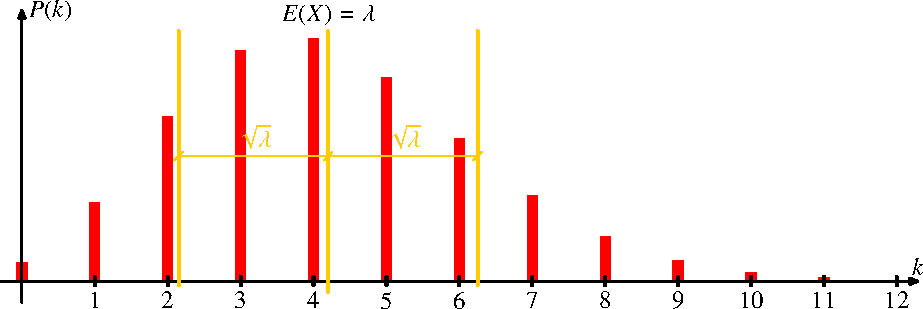
\includegraphics{images/exp-2.pdf}
\caption{Wahrscheinlichkeitsverteilung der Poisson-Verteilung f"ur
$\lambda=4.2$, $E(X)=\lambda$ und $\operatorname{var}(X)=\sqrt{\lambda}$.
\label{poisson-verteilung}}
\end{figure}
\begin{table}
\renewcommand{\arraystretch}{1.5}
\begin{center}
\begin{tabular}{|l|l|}
\hline
Name&Poissonverteilung\\
\hline
Wahrscheinlichkeit&
\begin{minipage}{3.7in}
\vskip3pt
$\displaystyle
P_\lambda(k)=\frac{\lambda^k}{k!}e^{-\lambda}
$
\end{minipage}
\\
Erwartungswert&$\displaystyle \lambda$\\
Varianz&$\displaystyle \lambda$\\
\hline
Anwendungen&\begin{minipage}{3.7in}%
\vskip3pt
\strut
$\bullet$ Anzahl Ereignisse mit exponentialverteilten Intervallen\\
$\bullet$ Approximation der Binomialverteilung f"ur seltene Ereignisse, die
mit Rate $\lambda$ eintreten
\strut
\end{minipage}\\[20pt]
\hline
\end{tabular}
\end{center}
\caption{Datenblatt der Poissonverteilung\label{datenblatt:poissonverteilung}}
\end{table}
Die Poissonverteilung liefert eine Antwort auf folgende Frage. In Abschnitt
\ref{section-exponentialverteilung} wurde die Exponentialverteilung
als die Verteilung f"ur die Ausfallwahrscheinlichkeit eines ``ged"achtnislosen''
Bauteils vorgestellt. Wir nehmen nun an, dass das Bauteil bei jedem Defekt
sofort ersetzt wird, und fragen danach, wie wahrscheinlich es ist, dass
wir in einem bestimmten Zeitintervall $k$ Ausf"alle beobachten.

Sei $X_i$ die Lebensdauer des Bauteils mit der Nummer $i$, es handelt
sich dabei um eine exponentialverteilte Zufallsvariable. Wenn im Zeitintervall
$[0,x]$ genau $k$ Ausf"alle beobachtet wurden, dann heisst das, dass die
Summe von $k$ Zufallsvariablen $\le x$ ist, jene von $k+1$ Zufallsvariable
aber $>x$. Also
\[
P(X_1+\dots+X_k\le x \wedge X_1+\dots+X_{k+1}>x)
\]
Wir berechnen diese Wahrscheinlichkeit in zwei Schritten.

Zun"achst interessiert uns, wie gross die Wahrscheinlichkeit ist, dass im
Intervall $[0,x]$ mindestens $k$ Ausf"alle passieren, dies ist
$P(X_1+\dots+X_k\le x)=F_{X_1+\dots+X_k}(x)$, also die Verteilungsfunktion
einer Summe von $k$ identisch exponentialverteilten Zufallsvariablen. Wir
behaupten:
\begin{satz}Sind $(X_i)_{1\le i\le k}$ identische exponentialverteilte,
unabh"angige Zufallsvariablen, dann hat deren Summe folgende Verteilungsfunktion
und Wahrscheinlichkeitsdichte:
\begin{eqnarray*}
F_{X_1+\dots+X_k}(x)&=&\begin{cases}
{\displaystyle 1-e^{-ax}\sum_{i=0}^{k-1}\frac{(ax)^i}{i!}}&\qquad x \ge 0\\
0&\qquad x < 0
\end{cases}
\\
\varphi_{X_1+\dots+X_k}(x)&=&\begin{cases}
{\displaystyle a^k\frac{x^{k-1}}{(k-1)!}e^{-ax}}&\qquad x\ge0\\
0&\qquad x < 0\end{cases}
\end{eqnarray*}
\end{satz}
\begin{proof}[Beweis]
Wir beweisen zun"achst die Formeln f"ur die Dichtefunktion $\varphi_k$ mit
Hilfe von vollst"andiger Induktion. F"ur $k=1$ liegt nur eine einzige
Zufallsvariable vor, durch Einsetzen von $k$ finden wir f"ur $x>0$
\[
\varphi_1(x)=ae^{-ax},
\]
also genau die Dichte der Exponentialverteilung. Offensichtlich ist dies
die richtige Wahrscheinlichkeitsdichte.

Wir nehmen nun an, dass obige Formel die Wahrscheinlichkeitsdichte f"ur die
Summe von $k$ Zufallsvariablen korrekt ist, und berechnen die daraus
folgende Wahrscheinlichkeitsdichte f"ur eine Summe von $k+1$ Zufallsvariablen.
Dazu wird die Faltung verwendet, es gilt f"ur $x>0$
\begin{eqnarray*}
\varphi_k*\varphi_1(x)
&=&
\int_{-\infty}^{\infty}\varphi_k(t)\varphi_1(x-t)\,dt\\
&=&\int_0^x a^k\frac{t^{k-1}}{(k-1)!}e^{-at}ae^{-a(x-t)}\,dt\\
&=&a^{k+1}e^{-ax}\int_0^x \frac{t^{k-1}}{(k-1)!}\,dt\\
&=&a^{k+1}e^{-ax}\left[\frac{t^k}{k!}\right]_0^x\\
&=&a^{k+1}e^{-ax}\frac{x^k}{k!}=\varphi_{k+1}(x)
\end{eqnarray*}
Damit ist die Formel f"ur $\varphi_k$ f"ur alle $k$ gezeigt.

Aus der Wahrscheinlichkeitsdichte kann nun auch die Verteilungsfunktion
berechnet werden. Durch partielle Integration kann man die Verteilungsfunktion
wie folgt berechnen:
\begin{eqnarray*}
F_k(x)
&=&\int_0^x\varphi_k(t)\,dt\\
&=&\int_0^xa^k\frac{t^{k-1}}{(k-1)!}e^{-at}\,dt\\
&=&\left[-a^{k-1}\frac{t^{k-1}}{(k-1)!}e^{-at}\right]_0^x+\int_0^xa^{k-1}\frac{t^{k-2}}{(k-2)!}e^-at\,dt\\
&=&-a^{k-1}\frac{x^{k-1}}{(k-1)!}e^{-ax}+F_{k-1}(x)\\
&=&-\frac{(ax)^{k-1}}{(k-1)!}e^{-ax}+F_{k-1}(x)
\end{eqnarray*}
Die Verteilungsfunktion $F_1$ von $\varphi_1$ kennen wir bereits:
\[
F_1(x)=\int_0^xae^{-at}\,dt=-e^{-ax}+1.
\]
Daraus leiten wir ab
\[
F_k(x)=1-e^{-ax}\sum_{i=0}^{k-1}\frac{(ax)^i}{i!}
\]
Die Summe ist die Partialsumme f"ur die Reihenentwicklung von $e^{ax}$,
insbesondere ist die Partialsumme immer kleiner als $a^{ax}$, also
\[
e^{-ax}\sum_{i=0}^{k-1}\frac{(ax)^i}{i!}<e^{-ax}\cdot e^{ax}=1,
\]
und damit $F_k(x) \le 0$. Andererseits ist die Partialsumme nur ein
Polynom in $x$, welches niemals so schnell wachsen kann wie $e^{-ax}$ kleiner
wird. Im Grenzwert $x\to\infty$ verschwindet der zweite Summand daher und
es gilt wie zu erwarten ist $\lim_{x\to\infty}F_k(x)=1$.
\end{proof}
Die hier gefundenen Verteilungen sind auch von einiger praktischer Bedeutung,
sie heissen die Erlang-Verteilungen.
\index{Erlang-Verteilung}

Um nun die Wahrscheinlichkeit $P_k(x)$ des Auftretens von genau $k$ Ausf"allen
ist jetzt also die Wahrscheinlichkeit, dass bis zur Zeit $x$ mindestens
$k$ Ausf"allen aufgetreten sind minus die Wahrscheinlichkeit, dass mehr
als $k$ Ausf"alle aufgetreten sind: 
\[
P_k(x)=P(\text{mindestens $k$ Ausf"alle})-P(\text{mehr als $k$ Ausf"alle})
\]
Die Wahrscheinlichkeit von mehr als $k$ Ausf"allen ist aber die Wahrscheinlichkeit
von mindestens $k+1$ Ausf"allen, also
\begin{eqnarray*}
P_k(x)&=&P(\text{mindestens $k$ Ausf"alle})-P(\text{mindestens $k+1$ Ausf"alle})\\
&=&F_k(x)-F_{k+1}(x)\\
&=&1-e^{-ax}\sum_{i=0}^{k-1}\frac{(ax)^i}{i!}-1+e^{-ax}\sum_{i=0}^{k}\frac{(ax)^i}{i!}\\
&=&e^{-ax}\frac{(ax)^k}{k!}
\end{eqnarray*}
Somit haben wir die Wahrscheinlichkeit berechnet, dass im betrachteten
Intervall genau $k$ Bauteile versagen.
Dies f"uhrt uns zur Definition der Poissonverteilung:
\begin{definition} Die Poissonverteilung
\[
P_\lambda(k)=\frac{\lambda^k}{k!}e^{-\lambda}
\]
beschreibt f"ur $\lambda=ax$ die Wahrscheinlichkeit,
dass in einem Zeitintervall $[0,x]$ genau $k$ Ereignisse eintreten, wenn
die Zeit zwischen den Ereignissen exponentialverteilt ist mit Dichte
$ae^{-ax}$.
\end{definition}

\subsubsection{Erwartungswert und Varianz}
\index{Poissonverteilung!Erwartungswert}
\index{Poissonverteilung!Varianz}
\index{Erwartungswert!Poissonverteilung}
\index{Varianz!Poissonverteilung}
Mit Hilfe der geschlossenen Formel f"ur die Poissonverteilung kann man
jetzt auch Erwartungswert und Varianz berechnen:
\begin{eqnarray*}
E(X)&=&\sum_{k=0}^\infty kP_\lambda(k)\\
&=&\sum_{k=0}^\infty k\frac{\lambda^k}{k!}e^{-\lambda}\\
&=&\lambda e^{-\lambda}\sum_{k=1}^\infty\frac{\lambda^{k-1}}{(k-1)!}\\
&=&\lambda e^{-\lambda}\sum_{k=0}^\infty\frac{\lambda^k}{k!}\\
&=&\lambda e^{-\lambda}e^\lambda=\lambda\\
\end{eqnarray*}
F"ur $E(X^2)$ finden wir analog
\begin{eqnarray*}
E(X^2)&=&\sum_{k=0}^\infty k^2P_\lambda(k)\\
&=&\sum_{k=0}^\infty k^2\frac{\lambda^k}{k!}e^{-\lambda}\\
&=&\lambda e^{-\lambda}\sum_{k=1}^\infty k\frac{\lambda^{k-1}}{(k-1)!}\\
&=&\lambda e^{-\lambda}\frac{d}{d\lambda}\sum_{k=1}^\infty \frac{\lambda^k}{(k-1)!}\\
&=&\lambda e^{-\lambda}\frac{d}{d\lambda}\lambda\sum_{k=1}^\infty \frac{\lambda^{k-1}}{(k-1)!}\\
&=&\lambda e^{-\lambda}\frac{d}{d\lambda}\lambda e^{\lambda}\\
&=&\lambda e^{-\lambda}(e^\lambda+\lambda e^\lambda)\\
&=&\lambda(1+\lambda)
\end{eqnarray*}
Daraus erhalten wir die Varianz:
\[
\operatorname{var}(X)=E(X^2)-E(X)^2=\lambda^2+\lambda -\lambda^2 =\lambda.
\]
\begin{satz}
Die Poissonverteilung $P\lambda(k)$ hat Erwartungswert
$E(X)=\lambda$ und Varianz $\operatorname{var}(X)=\lambda$.
\end{satz}

\subsubsection{Poissonverteilung als Approximation f"ur die Binomialverteilung}
\index{Poissonverteilung!Approximation der Binomialverteilung}
Das folgende Experiment soll diese Anwendung motivieren: 18 mal werden zwei 
W"urfel geworfen, und in einem $6\times 6$-Feld das Feld mit der
erw"urfelten Zeilen- und Spalten-Nummer angekreuzt. Dabei muss man darauf
achten, immer den gleichen W"urfel f"ur die Zeilen-Nummern zu verwenden.
Dann wird ausgez"ahlt, wieviele Felder $k=0$, $k=1$, $k=2$,\dots\ Kreuze
enthalten.

Nat"urlich ist dies ein Bernoulli-Experiment. Die Wahrscheinlichkeit, ein
bestimmtes Feld anzukreuzen, ist $p=\frac{1}{36}$, das Experiment
wird $18$ mal wiederholt. Die Wahrscheinlichkeit $P(k)$, dass das Feld $k$ mal
angekreuzt wurde, ist durch die Binomialverteilung gegeben:
\[
P(k)=\binom{n}{k}p^k(1-p)^{n-k}.
\]

Leider ist dieser Ausdruck f"ur grosses $n$ schwierig auszurechnen.
Wir suchen also nach einer Approximation, die leichter auszuwerten ist.
Dabei k"onnen wir nicht einfach $n\to\infty$ gehen lassen, denn die
Wahrscheinlichkeit $P(k)$ w"urde dann auch anwachsen. Wir m"ussen
gleichzeitig die Wahrscheinlichkeit kleiner machen, so dass die Rate $\lambda$,
mit der Kreuze gemacht werden, gleich bleibt. Im Experiment wird
die H"alfte ($\lambda=\frac{18}{36}=\frac12$) der Felder angekreuzt.
Die Wahrscheinlichkeit $p$ muss also mit $\lambda$ "uber die Formel
\[
p=\frac{\lambda}{n}
\]
zusammenh"angen.

\begin{figure}
\begin{center}
\begin{tabular}{|r|r|r|r|r|}
\hline
$k$&Binomial&empirisch&Poisson&\\
\hline
0&   0.60440867 & 0.60226943 & 0.60653066 & 21.8351 \\
1&   0.30646073 & 0.30971007 & 0.30326533 & 10.9176 \\
2&   0.07553610 & 0.07521756 & 0.07581633 &  2.7294 \\
3&   0.01205740 & 0.01146811 & 0.01263606 &  0.4549 \\
4&   0.00140104 & 0.00123035 & 0.00157951 &  0.0569 \\
5&   0.00012629 & 0.00009816 & 0.00015795 &  0.0057 \\
6&   0.00000919 & 0.00000599 & 0.00001316 &  0.0005 \\
7&   0.00000055 & 0.00000031 & 0.00000094 &  0.0000 \\
8&   0.00000003 & 0.00000002 & 0.00000006 &  0.0000 \\
9&   0.00000000 & 0.00000000 & 0.00000000 &  0.0000 \\
\hline
\end{tabular}
\end{center}
\caption{Wahrscheinlichkeit, in einem $6\times 6$-Feld nach 18-maligem
zuf"alligem Ankreuzen eines Feldes gefunden Verteilung der Anzahl Kreuze.
Die Spalte ganz rechts enth"alt die erwartet Anzahl Felder mit $k$ Kreuzen.
\label{cross36}}
\end{figure}

Damit kann man jetzt die Approximation durchf"uhren:
\begin{align*}
\binom{n}{k}p^k(1-p)^{n-k}
&=
\frac{n(n-1)(n-2)\dots(n-k+1)}{k!}\cdot \biggl(\frac{\lambda}n\biggr)^k\cdot \biggl(1-\frac{\lambda}n\biggr)^{n-k}\\
&=
\frac{\lambda^k}{k!}
\cdot\frac{n}{n}
\cdot\frac{n-1}{n}
\cdot\frac{n-2}{n}
\dots
\cdot\frac{n-k+1}{n}
\cdot
\biggl(1-\frac{\lambda}n\biggr)^n
\cdot
\biggl(1-\frac{\lambda}n\biggr)^{-k}
\end{align*}
F"ur $n\to\infty$ strebt der letzte Term gegen $1$.
Der zweitletzte Term strebt gegen $e^{-\lambda}$.
Jeder der Faktoren $\frac{n-i}n$ strebt gegeben $1$, und es sind ja nur
$k$ solche Faktoren, $k$ bleibt w"ahrend des Grenz"ubergangs unver"andert.
Daraus leiten wir ab:
\[
\lim_{n\to\infty} 
\binom{n}{k}p^k(1-p)^{n-k}
=
\frac{\lambda^k}{k!}e^{-\lambda}=P_{\lambda}(k),
\]
die Poisson-Verteilung zum Parameter $\lambda$.

Wenden wir dies auf das urspr"ungliche Experiment an, also $n=36$,
$\lambda=0.5$, finden wir die Resultate in Tabelle~\ref{cross36}. 
Die Abweichungen in der Spalte der empirischen Resultate kommt "ubrigens
nicht daher, dass zu wenige Versuch gemacht worden w"aren, sondern daher,
dass wir jeweils immer alle Felder ausgez"ahlt haben. Diese sind aber nicht
unabh"angig. Die beim Ausz"ahlen des $6\times 6$-Feldes gefundenen Werte
sind also gar nicht die Resultate von $n$ unabh"angigen Bernoulli-Experimenten.
